\documentclass[
	% -- opções da classe memoir --
	12pt,				% tamanho da fonte
	openany,			% capítulos começam em pág ímpar (insere página vazia caso preciso)
  oneside,      % para impressão em página única. Oposto ao twoside (Nunca habilitar os dois!)
	%twoside,			% para impressão em recto e verso. Oposto a oneside (Nunca habilitar os dois!)
	a4paper,			% tamanho do papel. 
	% -- opções da classe abntex2 --
	%chapter=TITLE,		% títulos de capítulos convertidos em letras maiúsculas
	%section=TITLE,		% títulos de seções convertidos em letras maiúsculas
	%subsection=TITLE,	% títulos de subseções convertidos em letras maiúsculas
	%subsubsection=TITLE,% títulos de subsubseções convertidos em letras maiúsculas
	% -- opções do pacote babel --
	english,			% idioma adicional para hifenização
	french,				% idioma adicional para hifenização
	spanish,			% idioma adicional para hifenização
	brazil				% o último idioma é o principal do documento
	]{abntex2}

% ---
% Pacotes básicos 
% ---
\usepackage{lmodern}			  % Usa a fonte Latin Modern			
\usepackage[T1]{fontenc}		% Selecao de codigos de fonte.
\usepackage[utf8]{inputenc} % Codificacao do documento (conversão automática dos acentos)
\usepackage{lastpage}			  % Usado pela Ficha catalográfica
\usepackage{indentfirst}    % Indenta o primeiro parágrafo de cada seção.
\usepackage{color}				  % Controle das cores
\usepackage{graphicx}			  % Inclusão de gráficos
\usepackage{subfig}         % Sub-figuras
\usepackage{microtype}      % para melhorias de justificação
\usepackage{textcomp}       % Adiciona símbolo de trademark e outros ao T1
\usepackage{array}          % Usado nas tabelas com \newline
\usepackage{multirow}       % Define tabelas multirow
\usepackage[outputdir=Gen]{minted}
\usepackage{listings}       % Program listings
\usepackage{lscape}         % 90-degree rotated images and tables
\usepackage{longtable}      % multiple pages tables
		
% ---
% Pacotes adicionais, usados apenas no âmbito do Modelo Canônico do abnteX2
% ---
\usepackage{lipsum}				% para geração de dummy text
% ---

% ---
% Pacotes de citações
% ---
\usepackage[brazilian,hyperpageref]{backref}	 % Paginas com as citações na bibl
\usepackage[alf]{abntex2cite}	% Citações padrão ABNT

% Copiado das configurações do LyX

%%%%%%%%%%%%%%%%%%%%%%%%%%%%%% LyX specific LaTeX commands.
%% Because html converters don't know tabularnewline
\providecommand{\tabularnewline}{\\}

%%%%%%%%%%%%%%%%%%%%%%%%%%%%%% User specified LaTeX commands.

% --- 
% CONFIGURAÇÕES DE PACOTES
% --- 

% ---
% Configurações do pacote backref
% Usado sem a opção hyperpageref de backref
\renewcommand{\backrefpagesname}{Citado na(s) página(s):~}
% Texto padrão antes do número das páginas
\renewcommand{\backref}{}
% Define os textos da citação
\renewcommand*{\backrefalt}[4]{
	\ifcase #1 %
		Nenhuma citação no texto.%
	\or
		Citado na página #2.%
	\else
		Citado #1 vezes nas páginas #2.%
	\fi}%
% ---

% --- 
% NOME DA BASE
% --- 

% ---
% Nome da base
\newcommand{\databaseName}{Sorveteria}
\newcommand{\storeName}{Gelatto Felice}
\newcommand{\storeFullName}{Sorveteria \storeName{}}
% ---


% ---
% Informações de dados para CAPA e FOLHA DE ROSTO
% ---
\titulo{Resenha: "La tomada de decisiones de Directivos Latinos"}

\autor{André Ferreira Bem Silva}

\local{São Paulo, SP}
\data{09/04/2017}
\instituicao{%
  Fundação Getúlio Vargas -- FGV
  \par
  MBA Executivo em Economia e Gestão: Business Analytics e Big Data T3
  \par
  Disciplina de Decisões Empresariais e Raciocínio Analítico
}
\tipotrabalho{Resenha}
% O preambulo deve conter o tipo do trabalho, o objetivo, 
% o nome da instituição e a área de concentração 
\preambulo{Este trabalho é uma resenha e opinião a respeito do artigo "La tomada de decisiones de Directivos Latinos", sobre diferentes linhas de raciocínio em decisões de gerentes norte-americanos, europeus e sul americanos.}
% ---


% ---
% Configurações de aparência do PDF final

% alterando o aspecto da cor azul
\definecolor{blue}{RGB}{41,5,195}

% informações do PDF
\makeatletter
\hypersetup{
     	%pagebackref=true,
		pdftitle={\@title}, 
		pdfauthor={\@author},
    	pdfsubject={\imprimirpreambulo},
	    pdfcreator={LaTeX with abnTeX2},
		pdfkeywords={abnt}{latex}{abntex}{abntex2}{trabalho acadêmico}, 
		colorlinks=true,       		% false: boxed links; true: colored links
    	linkcolor=blue,          	% color of internal links
    	citecolor=blue,        		% color of links to bibliography
    	filecolor=magenta,      		% color of file links
		urlcolor=blue,
		bookmarksdepth=4
}
\makeatother
% --- 

% --- 
% Espaçamentos entre linhas e parágrafos 
% --- 

% O tamanho do parágrafo é dado por:
\setlength{\parindent}{1.3cm}

% Controle do espaçamento entre um parágrafo e outro:
\setlength{\parskip}{0.2cm}  % tente também \onelineskip

% ---
% compila o indice
% ---
\makeindex
% ---

% ----
% Início do documento
% ----
\begin{document}

% Seleciona o idioma do documento (conforme pacotes do babel)
%\selectlanguage{english}
\selectlanguage{brazil}

% Retira espaço extra obsoleto entre as frases.
\frenchspacing 

% ----------------------------------------------------------
% ELEMENTOS PRÉ-TEXTUAIS
% ----------------------------------------------------------
% \pretextual

% ---
% Capa
% ---
\imprimircapa
% ---

% ---
% Folha de rosto
% (o * indica que haverá a ficha bibliográfica)
% ---
\imprimirfolhaderosto
% ---

% ---

% ---

% ---

% ---
% inserir lista de ilustrações
% ---
%\pdfbookmark[0]{\listfigurename}{lof}
%\listoffigures*
%\cleardoublepage
% ---

% ---
% inserir lista de tabelas
% ---
\pdfbookmark[0]{\listtablename}{lot}
%\listoftables*
\cleardoublepage
% ---

% ---
% inserir lista de abreviaturas e siglas
% ---
%\begin{siglas}
%  \item[ABNT] Associação Brasileira de Normas Técnicas
%  \item[abnTeX] ABsurdas Normas para TeX
%\end{siglas}
% ---

% ---
% inserir lista de símbolos
% ---
%\begin{simbolos}
%  \item[$ \Gamma $] Letra grega Gama
%  \item[$ \Lambda $] Lambda
%  \item[$ \zeta $] Letra grega minúscula zeta
%  \item[$ \in $] Pertence
%\end{simbolos}
% ---

% ---
% inserir o sumario
% ---
\pdfbookmark[0]{\contentsname}{toc}
\tableofcontents*
\cleardoublepage
% ---



% ----------------------------------------------------------
% ELEMENTOS TEXTUAIS
% ----------------------------------------------------------
\textual

% ----------------------------------------------------------
% Introdução (exemplo de capítulo sem numeração, mas presente no Sumário)
% ----------------------------------------------------------
%\chapter*[Introdução]{Introdução}
%\addcontentsline{toc}{chapter}{Introdução}
% ----------------------------------------------------------

\graphicspath{{./Gen/Image/}{../Gen/Image/}{./Image/}}

%Adiciona introdução com numeração
\chapter[Resenha]{Resenha}
Nesta seção discute-se a respeito dos pontos do artigo tema deste trabalho de maneira
científica e crítica. Fazendo-se assim uma tomada impessoal do que é descrito no mesmo.

\section{Questionamentos Principais}
\begin{enumerate}
\item Quais são os pontos mais interessantes do artigo na sua opinião?
\item Com quais pontos você concorda e quais discorda e por quê?
\item Apresente exemplos de situações que ilustrem a resposta do item anterior.
\item Após ler o artigo o que você mudaria em seu grupo ou sugeriria que
fosse mudado no seu grupo de trabalho ou na empresa? Por quê?
\end{enumerate}

\section{Resenha Sobre o Artigo}

O artigo referente a esta resenha trata das diferenças entre mecanismos
de gestão e tomada de ação relacionadas a diferenças culturais entre
norte-americanos, europeus e sul americanos, partindo do pressuposto
que todos agiriam de maneira similar ao serem defrontados com a uma
situação decisória complexa. Percebe-se pelo artigo que isso não acontece
na prática. 

Para isso, apresenta-se um problema complexo baseado em uma situação
real em uma empresa, em duas diferentes situações. O problema apresentado
acontece quando o chefe de divisão de uma empresa que tem quatro divisões
é apresentado uma petição do diretor geral para que sua divisão alcance
resultados que ele considerou inalcançáveis. Apesar de resistir um
pouco às metas traçadas pelo diretor geral, o gestor aceita o plano
dado que o diretor geral está obstinado as novas metas.

As metas foram apresentadas aos gerentes do chefe de divisão, os quais
contestam a meta imposta como impossível também. Entretanto, seus
pedidos de revisão das mesmas não foram atendidos. Sendo assim, o
gerente de vendas começou a impor vendas forçadas aos clientes de
diversas maneiras e o gerente de produção começou a falsificar faturas,
transformando gastos em ativos amortizáveis. Havia ainda um terceiro
funcionário que assim como o chefe de divisão não percebe o que está
acontecendo com as equipes dos gerentes.

Após meses batendo as metas de maneira irregular, a situação tornou-se
insustentável e os gerentes se reunem com o chefe e contam tudo. O
chefe de divisão então teve em suas mãos um problema complexo. Sabia
que o diretor geral, seu chefe, duvidava da sua capacidade de coordenar
a situação e bater as metas. Então questionou-se o que deveria fazer?
Contava a ele tudo ou tentaria esboçar um plano de contenção antes
de fazê-lo?

A partir desse problema complexo constrói-se, colocando-se esse problema
para setecentos diferentes gestores ao redor do mundo. Observando-se
a resposta dos mesmos o artigo observou que houve uma tendência a
encontrar-se uma saída por demitir-se um dos funcionários infratores
como \emph{bode expiatório}. Alguns teriam levado o tema direto ao
diretor geral, com a renúnica pessoal (da posição de chefe de divisão).
Em geral, a maioria resistiu a demitir todos os funcionários envolvidas
para não deixar a empresa sem recursos. Nenhum gestor, nem no primeiro,
nem no segundo experimento sugeriu a possiblidade de voltar ao diretor
geral e questionar-se as metas aplicadas inicialmente e suas consequências.
Este é um ponto chave do artigo, uma vez que não houve um questionamento
do que haveria gerado o problema inicial. 

Inicia-se o artigo com a contextualização do mesmo com a informação
de que situações complexas envolvem capacidade de raciocínio analítico
além daquilo que uma pessoa pode pensar em um curto espaço de tempo
e que as ferramentas tecnológicas que dispõe-se hoje em dia para avaliar
uma situação são o sonho de qualquer gestor na tomada de decisão.
Isso é uma linha de pensamento alinhada a gestão moderna baseada no
suporte tecnológico para o mecanismo de tomada de decisão.

O que parece é que a decisão de tomada de decisão referente ao caso
do artigo é que não há uma racionalidade por trás da decisão de aumento
de metas, ou mesmo uma transparência profunda por parte do diretor
geral e do chefe de divisão com os demais funcionários da empresa,
sendo uma decisão que foi tomada de maneira hierárquica sem haver
muita discussão sobre sua real viabilidade. Por isso, o resultado
esperado não poderia ser outro? 

É surpreendente a análise do segundo exemplo, quando a equipe de gestores
norte-americanos chega a conclusão de que o culpado só poderia ser
os funcionários que faltaram com ética e tentaram bater a meta a qualque
custo, após apenas 15 minutos de discussão. Parece que houve uma decisão
muito rasa com relação aquilo que poderia ter levado os funcionários
a um comportamento extremo. Talvez, elucida-se a maneira como muitas
decisões são tomadas em empresas norte-americanas e ao redor do mundo,
não tendo a visão do todo, como relata-se no artigo.

Cada funcionário tenderia a ver o problema com sua visão de especialista
que seria uma visão do problema sob determinada ótica. Essa ótica
enxergaria somente parte da verdade. Um problema complexo é a soma
de diversos problemas pontuais acrescentados de tempo. Somente a racionalidade
e o acesso a informação pode torná-los mais compreensíveis. Por isso,
muitas vezes prefere-se postergar a decisão final por falta de informação
a respeito da questão a ser resolvida. Ainda assim, isso tende a ser
uma armadilha, conforme mencionado no artigo. O que não fica mencionado
é que talvez fosse mais interessante tomar a decisão de maneira compartilhada,
baseada em informações obtidas com os dados da própria empresa.

As ferramentas tecnológicas de suporte a decisão encontram-se disponíveis,
é o chamado \emph{big data}. É possível por meio dela obter-se as
informações básicas para entender-se o problema inicial nesse caso.
Isto é, se as metas definidas pelo diretor geral seriam razoáveis
dado a situação atual da empresa e sua possível expansão de mercado.
Assim, teria-se uma visão holística de como é a situação atual na
empresa e poderia-se ter uma previsão realista de para onde a empresa
poderia ir. No popular, \emph{contra números não há argumentos}. E
realmente, espera-se que uma decisão de aumento na meta de vendas
da empresa tem que ser embasada na realidade, ou as consequências
podem ser exatamente como as observadas nesse caso.



\chapter[Reflexão]{Reflexão}
Neste capítulo será discutido reflexões em tom pessoal a respeito do que 
poderia ser feito relacionado ao tema da resenha tema deste artigo.

\section{Reflexão Individual Quanto à Organização Siemens Healthineers}

Após a leitura do trabalho evidencia-se, em minha opinião, que muito
do que foi dito é válido para a empresa a qual trabalho como colaborador,
a Siemens Healthineers. Digo isso, em função de muitas das decisões
a serem tomadas envolvem fatores complexos e os números que dão base
a esse processo decisório nem sempre estão disponíveis facilmente.

Por isso, o acesso a informação e seu processamento contínuo deve
fazer parte de uma organização. Creio também que a tomada de decisão
deve ser transparente. No exemplo citado no artigo, por exemplo, imagina-se
que o ambiente na empresa em questão seria muito tóxico durante o
ocorrido, pelo falto de haver pouca ciência por parte dos chefes com
relação a situação dos funcionários que trabalham efetivamente com
os clientes e os fornecedores. 

A fachada da empresa com os clientes e fornecedores é justamente os
funcionários em questão, e por isso, faz-se necessário observá-los
de perto. O fato de que problemas ficaram escondidos por muito tempo
do chefe de divisão, indica que havia pouca ou nenhuma comunicação
com os funcionários envolvidos e fica claro pela própria definição
do problema que seus problemas e contestações foram ignorados. 

Assim, acredito que mecanismos de feedback e observação constante
na empresa em qual trabalho seriam muito interessante para evitar
que esse tipo de problema aconteça e para que haja transparência e
confiança nas relações interpessoais na mesma.

% ----------------------------------------------------------
% Finaliza a parte no bookmark do PDF
% para que se inicie o bookmark na raiz
% e adiciona espaço de parte no Sumário
% ----------------------------------------------------------
\phantompart

% ---
% Conclusão - Recomendação de qual protótipo
% ---
%\chapter{Conclusões}
% ---

%Placeholder
%\label{chap:conclusao}

\begin{figure}
\begin{centering}
\subfloat[\label{fig:prototipo-familia}Conforto,
espaço e filhos.]{\begin{centering}
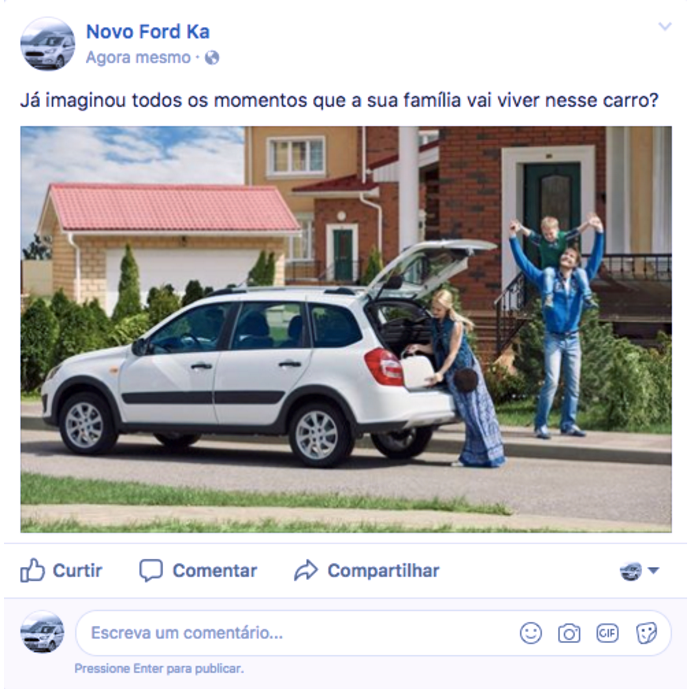
\includegraphics[height=0.30\textheight]{Imagens/p1_familia}~~
\par\end{centering}
}\subfloat[\label{fig:prototipo-versatil}Aborda o efeito versátil do carro.]{\begin{centering}
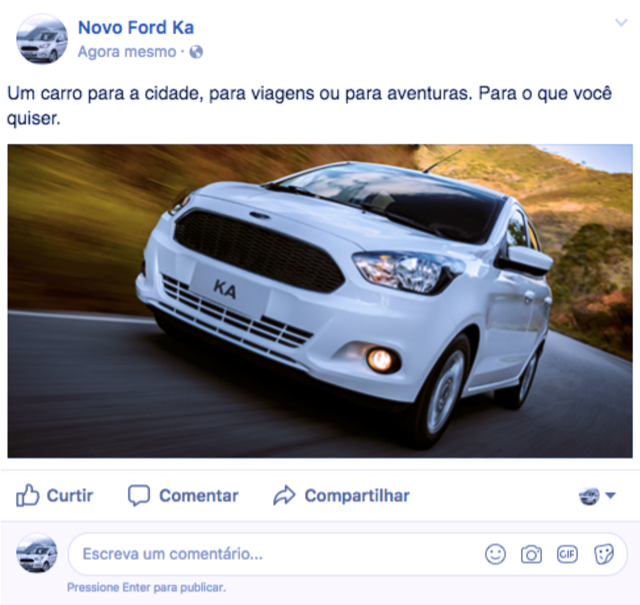
\includegraphics[height=0.30\textheight]{Imagens/p1_prototipo}
\par\end{centering}
}
\par\end{centering}
\caption{Peças ilustrativas de uma campanha em formato carrossel.}
\end{figure}

De acordo com o desenvolvido no capítulo \ref{chap:analise}, com
as tabelas \ref{tab:prototipo-vs-cluster} e \ref{tab:prototipo-analise},
contrasta a homogeneidade dos protótipo 2 e 3 à heterogeneidade do
protótipo 1. À primeira vista, percebe-se que os três protótipos possuem
proporções da população muito parecidas, entretanto há uma grande
diferença entre o protótipo 1, heterogêneo, com os demais protótipos.
Isto é, a possibilidade de uma campanha publicitária informativa unida
a transformativas que possibilitarão, se escolhido o protótipo 1,
abranger também os clusters \nomeCc{} e \nomeCb{}, dado que pela
própria heterogeneidade do protótipo 1, certas propagandas que apelam
para determinadas características do protótipo podem aumentar a aceitação
de uma campanha baseada neste protótipo.

\begin{table}
\begin{centering}
\begin{tabular}{c|>{\centering}p{0.28\textwidth}|>{\centering}p{0.28\textwidth}|>{\centering}p{0.28\textwidth}}
\hline 
 & Protótipo 1 & Protótipo 2 & Protótipo 3\tabularnewline
\hline 
Bom & Preferido entre \nomeCa{} e \nomeCd{}. & Amplamente preferido pelo cluster dos \nomeCc{}. & Amplamente preferido pelos \nomeCb{}, focados em Imagem.\tabularnewline
\hline 
Ruim & Somente uma estratégia de marketing não é suficiente, dada a sua heterogeneidade
e várias afinidades. & Difícil para a publicidade porque se mostra indiferente a carros.
Importam-se apenas com o preço. & Uma campanha publicitária em Imagem somente não gera interesse de
outros clusters.\tabularnewline
\hline 
\end{tabular}
\par\end{centering}
\caption{\label{tab:prototipo-analise}Vantagens e desvantagens por protótipos.}
\end{table}


Por exemplo, se uma campanha publicitária apelar de maneira informativa
e transformativa para os aspectos de Imagem e Utilitário do carro,
é possível abranger os clusters mencionados anteriormente, sustentando
assim uma aceitação maior por parte da população. Ou seja, escolhe-se
a versatilidade do protótipo 1, numa eventual campanha publicitária
como elemento.

\begin{figure}
\begin{centering}
\subfloat[\label{fig:painel-cambio}Acabamento e câmbio.]{\begin{centering}
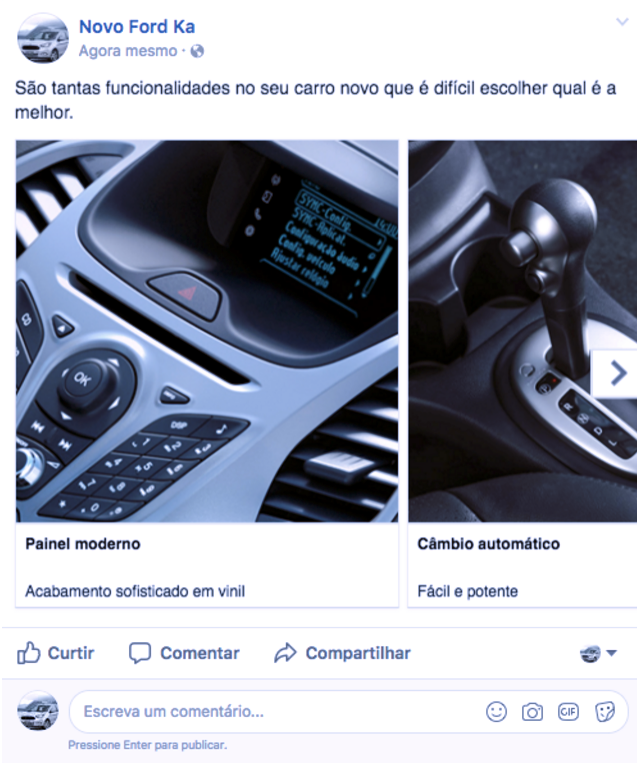
\includegraphics[height=0.34\textheight]{Imagens/p1_interior}
\par\end{centering}
}~~\subfloat[\label{fig:ar}Ar-condicionado.]{\begin{centering}
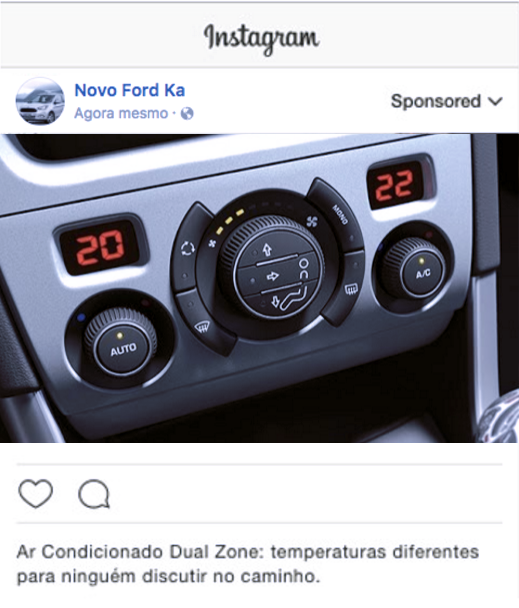
\includegraphics[height=0.34\textheight]{Imagens/p1_interior_painel}
\par\end{centering}
}
\par\end{centering}
\caption{Peças multifuncionais para Utilitário e Imagem.}
\end{figure}


\section{Recomendações para Campanha Publicitária}

Com base nas características analisadas dos grupos \nomeCa{} e \nomeCd{}
será feita uma combinação de campanhas publicitárias: para os \nomeCa{},
uma campanha transformativa mesclando os três atributos: Imagem, Utilitário
e Preço. Para os \nomeCd{}, uma campanha ressaltando o carro como
utilitário. Por se tratar de dois grupos diferentes vamos destacar
multifuncionalidade, tecnologia, versatilidade e conforto.

É possível uma campanh que foque nas seguintes características: confortável
e espaçoso. O público-alvo seriam os \nomeCd{} que preferem carros
como bens utilitários, destacando o porta-malas espaçoso para a família.
Os \nomeCd{} são formados predominantemente por mulheres com filhos,
por isso o destaque a família, na figura \ref{fig:prototipo-familia}.

A campanha com formato em carrossel irá abordar a característica de
multifuncionalidade. A publicidade tem foco nos \nomeCa{} combinando
funcionalidades (Utilitário) que valorizem o carro (Preço) e que tragam
mais sofisticação (Imagem), como vê-se nas figuras \ref{fig:painel-cambio}
e \ref{fig:ar}.

Finalmente, a figura \ref{fig:prototipo-versatil} seria veiculada
em formato vídeo, tanto em Facebook quanto na televisão. Destaca a
versatilidade do Ford Ka\texttrademark, valorizando o fato de ser
um carro potente (Utilitário) e ainda assim econômico (Preço). Em
televisão, dá-se preferência é por intervalos de jogos de futebol
buscando atingir um público predominantemente masculino que gosta
de esportes e aventuras. 



% ----------------------------------------------------------
% ELEMENTOS PÓS-TEXTUAIS
% ----------------------------------------------------------
\postextual
% ----------------------------------------------------------

% ----------------------------------------------------------
% Referências bibliográficas
% ----------------------------------------------------------
%\bibliography{referencias}

% ----------------------------------------------------------
% Glossário
% ----------------------------------------------------------
%
% Consulte o manual da classe abntex2 para orientações sobre o glossário.
%
%\glossary

% ----------------------------------------------------------
% Apêndices
% ----------------------------------------------------------

% ---
% Inicia os apêndices
% ---
%\begin{apendicesenv}

%% Imprime uma página indicando o início dos apêndices
%\partapendices

%% ----------------------------------------------------------
%\chapter{Quisque libero justo}
%% ----------------------------------------------------------

%\lipsum[50]

%% ----------------------------------------------------------
%\chapter{Nullam elementum urna vel imperdiet sodales elit ipsum pharetra ligula
%ac pretium ante justo a nulla curabitur tristique arcu eu metus}
%% ----------------------------------------------------------
%\lipsum[55-57]

%\end{apendicesenv}
% ---


% ----------------------------------------------------------
% Anexos
% ----------------------------------------------------------

% ---
% Inicia os anexos
% ---
%\begin{anexosenv}

%% Imprime uma página indicando o início dos anexos
%\partanexos

%% ---
%\chapter{Morbi ultrices rutrum lorem.}
%% ---
%\lipsum[30]

%% ---
%\chapter{Cras non urna sed feugiat cum sociis natoque penatibus et magnis dis
%parturient montes nascetur ridiculus mus}
%% ---

%\lipsum[31]

%% ---
%\chapter{Fusce facilisis lacinia dui}
%% ---

%\lipsum[32]

%\end{anexosenv}

%---------------------------------------------------------------------
% INDICE REMISSIVO
%---------------------------------------------------------------------
\phantompart
\printindex
%---------------------------------------------------------------------

\end{document}
